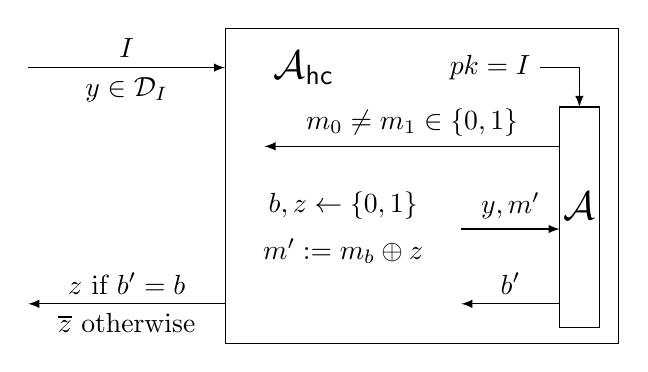
\begin{tikzpicture}
\draw (0,0) rectangle (5,4);
\draw (4.25,0.2) rectangle (4.75,3);
\draw[-latex] (-2.5,3.5) -- (0,3.5) node [midway, above] {$I$} node [midway, below] {$y \in \mathcal{D}_I$};
%\draw[-latex] (-2.5,2) -- (0,2) node [midway, above] {$g^3 = g^z$ or $g^{xy}$};
%\draw[-latex] (-2.5,1.5) -- (0,1.5) node [midway, above] {$c^2_b$};
\draw[-latex] (4,3.5) node [left] {$pk=I$} -| (4.5,3);
\draw[-latex] (0,0.5) -- (-2.5,0.5) node [midway, above] {$z$ if $b'=b$} node [midway, below] {$\overline{z}$ otherwise};
\draw (1,3.5) node {{\Large $\mathcal{A}_{\mathsf{hc}}$}};
\draw (4.5,1.75) node {\Large $\mathcal{A}$};
\draw[-latex] (4.25,2.5) -- (0.5,2.5) node [midway, above] {$m_0 \neq m_1 \in \{0,1\}$};
\draw (1.5,1.45) node [above] {$b,z \gets \{0,1\}$} node [below] {$ m' := m_b\oplus z$};
\draw[-latex] (3,1.45) -- (4.25,1.45) node [midway, above] {$y, m'$};
\draw[-latex] (4.25,0.5) -- (3,0.5) node [midway, above] {$b'$};
%\draw[-latex] (4.5,3.5) node[above] {$pk$} -- (4.5,3);
\end{tikzpicture}